\chapter{Verbindungsmittel}

Man unterscheidet zwischen metallischen Verbindungsmitteln (Drahtstifte, Schrauben, Verbindungsbeschläge) und nichtmetallischen Verbindungsmitteln (Klebstoffe, Leime, Dübel, Federn).\footnote{http://www.sign-lang.uni-hamburg.de/tlex/lemmata/l7/l708.htm,[06,2013]}



\section{Schrauben}





Die Idee war, eine Verbindung zwischen Holz und Beton herzustellen, welche die Schubkräfte abtragen kann und damit den Holzleichtbeton unterstützt. Analog zum herkömmlichen HBV - System, wurde gemeinsam mit Firma SFS das System mit langen Holzschrauben als Schubverbinder entwickelt. Die Festigkeit der Verbindungsmittel  (Verschiebungsmodul) beeinflusst das Trag- und Verformungsverhalten des nachgiebig verbundenen Sandwich-Elementes. Vorteil dieses Systems ist, dass die Schrauben ohne Vorbohren in das Holz eingebohrt werden können. Es gibt mehrere Hersteller, die in der Arbeit von Schernberger [1] aufgelistet sind, die dieses System anbieten. Es wird auch auf die Einsatzmöglichkeiten und die Vor- und Nachteile jedes Herstellers eingegangen. Die Firma hat Schraubenreihen  in verschiedensten Ausführungsvarianten und entsprechenden Schraubenlängen. Um die Auswahl der Schrauben einzugrenzen, wurden folgende Eigenschaften vorgegeben:


\begin{enumerate} 
	\item Einschraubwinkel: $45^{\circ}$
	\item Schraubenlänge: \unit[400]{mm} 
	\item Einschraubtechnik: ohne Vorbohren
	\item Keine Beschädigung der Schrauben beim durchbohren des Holzleichtbetons (Velox)
\end{enumerate}


Der vierte Punkt war aufgrund des Sandwichaufbaus noch nicht überprüft worden. Daher wurden in Zusammenarbeit mit der Firma SFS verschiedene Schraubentypen getestet. 

Die Schrauben unterschieden sich in: 

\begin{itemize}
	\item Schraubenkopfform
	\item Gewindeanordnung
	\item Schaftform
	\item Spitze
\end{itemize}

Ausgesuchte Schraubentypen: 


\begin{itemize}
	\item WR – dxL
	\item TWIN – DU dxL Sichel
	\item WT – T dxL 
	\item TWIN – DU dxL
	\item WR – T  dxL
\end{itemize}
	
\subsection{Schraubentype:	 WR – dxL}
Das Befestigungssystem WR findet hauptsächlich bei großen Querschnitten im Bereich der Verbindungen, Verstärkungen und Stahl-Holz-Anschlüsse, Anwendung. Die Schrauben sind aus Kohlenstoffstahl gefertigt. Der Schraubendurchmesser ist wählbar zwischen 9 mm oder 13 mm. Die Schrauben sind in den Längen von \unit[250]{mm} bis \unit[1000]{mm} verfügbar. Die Oberfläche der Schraube ist mit einem Durocoat überzogen, der als Korossionsschutz und als Gleitmittel fungiert.

\begin{figure}[h]
\begin{center}
\includegraphics[scale =0.7]{Verbindungsmittel/schrauben/WR-dxL.png}
\caption{Schraubentype: WR - dxL}
\end{center}
\end{figure}


\subparagraph{Positive Eigenschaften laut Hersteller[], sind:}

\begin{itemize}
	\item sehr hohe Leitungsfähigkeit
	\item breites Anwendungsspektrum
	\item Verschraubung auch paralell zur Faserrichtung möglich
	\item keine Abminderung der Tragfähigkeit von $90^\circ  -  45^\circ$ zur Faser
	\item Verarbeitung ohne Vorbohren
	\item geringe Spaltneigung
	\item unsichtbare Verbindung
\end{itemize}


\subsection{Schraubentype: TWIN-UD dxL Sichel }
Das System TWIN DU wird seit Jahren für die Befestigung von Aufsparrendämmung auf Dächern  und hinterlüftete Fassaden verwendet. Die Schrauben sind aus Kohlenstoffstahl gefertigt. Der Schraubendurchmesser beträgt \unit[7,5]{mm} und die Schraubenlänge variiert im Bereich von \unit[160]{mm} bis \unit[480]{mm}. Die Oberfläche der Schraube ist mit einem Durocoat überzogen, der als Korossionsschutz und als Gleitmittel fungiert.

\begin{figure}[h]
\begin{center}
\includegraphics[scale =0.7]{Verbindungsmittel/schrauben/TWIN-UDdxLSichel.png}
\caption{Schraubentype: TWIN-UD dxL Sichel}
\end{center}
\end{figure}


\subparagraph{Positive Eigenschaften nach Angaben des Herstellers [], sind:}

\begin{itemize}
	\item Holzbohrspitze reduziert die Spaltgefahr des 	Holzes
	\item optimiertes Doppelgewinde ohne		 Gangunterschied
	\item Rändel für erleichtertes Eindrehen
	\item mehr Leistung durch angepasste 	Gewindedurchmesser
	\item hohe Traglast auf Zug und Druck dank 	Doppelgewinde
	\item minimale Wärmebrücken bei vollflächiger 	Dämmung
	\item einfache Arbeitsschritte- minimaler 	Arbeitsaufwand
	\item Dämmstärken von \unit[60]{mm} bis \unit[300]{mm} möglich
\end{itemize}


\subsection{Schraubentype: WT – T dxL }
Das Befestigungssystem WT-T ist für den universellen Einsatz im konstruktiven Holzbau in Gebrauch. Die Schrauben sind aus Kohlenstoffstahl gefertigt. Der Schraubendurchmesser ist wählbar zwischen \unit[6,5]{mm} oder \unit[8,2]{mm}. Die Schrauben sind in den Längen von  \unit[65]{mm} bis \unit[330]{mm}verfügbar. Die Oberfläche der Schraube ist mit einem Durocoat überzogen, der als Korossionsschutz und als Gleitmittel fungiert.

\begin{figure}[h]
\begin{center}
\includegraphics[scale =0.7]{Verbindungsmittel/schrauben/WT-TdxL.png}
\caption{Schraubentype: WT-T dxL}
\end{center}
\end{figure}

\subparagraph{Positive Eigenschaften laut Hersteller[], sind:}

\begin{itemize}
	\item einfache und sichere Berechnung
	\item vielfältiges Anwendungsspektrum
	\item dauerhafte Verbindung  bei hoher Tragfähigkeit
	\item schnelles, effizientes Verarbeiten ohne Vorbohren
	\item formschlüssige Verbindung  dank Doppelgewinde
	\item hoher Brandwiderstand
	\item anspruchsvolle Ästhetik dank versenkter Befestigungsmittel
	
\end{itemize}

\subsection{Schraubentype:	 WR – T  dxL}
Das Befestigungssystem WR-T ist für den universellen Einsatz im konstruktiven Holzbau in Gebrauch. Die Schrauben sind aus Kohlenstoffstahl gefertigt. Der Schraubendurchmesser ist wählbar zwischen \unit[9]{mm} oder \unit[13]{mm}. Die Schrauben sind in den Längen von  \unit[250]{mm} bis \unit[1000]{mm} verfügbar. 

\begin{figure}[h]
\begin{center}
\includegraphics[scale =0.7]{Verbindungsmittel/schrauben/WR-TdxL.png}
\caption{Schraubentype: WT-T dxL}
\end{center}
\end{figure}

\subparagraph{Positive Eigenschaften nach Angaben des Herstellers [], sind:}

\begin{itemize}
	\item hohe Tragfähigkeit
	\item einfache Verarbeitung
	\item hoher Brandwiderstand der Verbindung
	\item schnelle Montage ohne Vorbohen
	\item Verbindungsmittel nicht sichtbar
\end{itemize}

\subsection{Versuchsaufbau für Schrauben}

Bei der Produktion werden zuerst die Holzbetonplatten auf die BSP geklebt und anschließend die Schrauben durch die Holzbetonplatten in die BSP eingeschraubt. Die Versuchsdurchführungen sollen sicher stellen, dass nach der Durchdringung der Holzleichtbetonschicht das Gewinde und die Spitze keinen Schaden nehmen und damit eine einwandfreie Verbindung im Holz zustande kommt. \newline Es wurden vier Lagen Veloxplatten zu je \unit[5]{cm} übereinandergelegt und mit Klemmzangen zusammengehalten. Um das Durchbohren und die anschließende Besichtigung der Schrauben zu ermöglichen, wurden die Platten auf Holzböcken gelagert.  

\begin{figure}
\begin{center}
\includegraphics[scale =0.6]{Verbindungsmittel/schrauben/Schraubenversuchsaufbau.png}
\caption{ Schraubenversuchsaufbau}
\end{center}
\end{figure}

\subsection{Versuchsauswertung}

In Abbildung \ref{Schraubenauswertung} sind die Schraubenspitzen nach dem Durchbohren der Veloxplatten dargestellt. Es ist ersichtlich, dass keine der Schrauben beschädigt worden ist. Weiters war beim Einbohren der Schrauben, kein Unterschied im Kraftaufwand festzustellen. \newline

\begin{figure}[h!]
\begin{center}
\includegraphics[scale =0.8]{Verbindungsmittel/schrauben/Schraubenauswertung.png}
\caption{ Schraubenansicht nach dem Durchbohren der vier Veloxplatten}
\label{Schraubenauswertung}
\end{center}
\end{figure}


Aufgrund der folgenden Kriterien wurde der Typ \textbf{WR – T 9\,x\unit[400]{mm}} ausgewählt.
Um über den gesamten Einbohrvorgang eine Führung zu gewährleisten, wurde eine Gewindeanordnung über die gesamte Schraubenlänge bevorzugt. Zusätzlich kann durch das Gewinde ein besserer Auszugswiderstand aus dem Beton gewährleistet werden. Die Bandbreite der Schraubenlänge beträgt \unit[250]{mm} bis \unit[1000]{mm}.
Die Spitze war ein weiteres Entscheidungskriterium, hierbei wurde darauf geachtet, dass sich die Schraube problemlos mit einem einfachen Hilfsmittel (Hammer) ansetzen lässt. 
Der Schraubenkopf besitzt eine große Fläche, somit wird ein guter  Verbund mit dem Beton erreicht. 





\section{Kleber}
Unter Kleben versteht man: Fügen gleicher oder ungleicher Werkstoffe unter Verwendung eines Klebstoffes.[(nach EN DIN 923,[])] 

Klebstoffe sind nichtmetallische Stoffe, die Fügeteile durch Flächenhaftung und innere Festigkeit(Adhäsion und Kohäsion) verbinden.(nach EN DIN 923,[])


\subsection{Einteilung}

Die Einteilung der Klebestoffe wird in Habenich[] auf zwei Arten angeführt. Zum einen auf der chemischen Basis und nach dem Abbindemechanismus. 
\begin{figure}[h]
\begin{center}
\includegraphics[scale =0.6]{Verbindungsmittel/kleber/einteilungderklebstoffe.png}
\caption{ Einteilung der Klebstoffe nach dem Abbindemechanismus, []}
\label{Einteilung der Kelbstoffe}
\end{center}
\end{figure}


\subsection{Vor- und Nachteile der Klebverbindungen}

Habenich [] hat die Vor- und Nachteile des Klebens gegenüber Schweißen, Löten, Schrauben, und Nieten beschrieben. 
\newline{}

\textbf{Vorteile von Klebungen,[4, Tabelle 7.1]}
\begin{itemize}
	\item gleichmäßige Spannungsverteilung senkrecht zur Belastungsrichtung 
	\item keine Thermische Gefügebeeinflussung
	\item kein thermisch bedingter Bauteilverzug
	\item Verbindungsmöglichkeit für unterschiedliche Materialkomponenten
	\item Gewichtsersparnis, Leichtbau
	\item Verbingungsmöglichkeit für sehr wärmeempfindliche Werkstoffe
	\item Festigkeitserhöhung in Verbindung mit Schrauben
	\item hohe dynamische Festigkeit, hohe Schwingunsdämpfung
	\item Möglichkeit zur Automatisierung
\end{itemize}


\textbf{Nachteile von Klebungen, [4, Tabelle 7.2]}

\begin{itemize}
	\item Einfluss der Zeit auf den Verfahrensablauf
	\item Oberflächenvorbehandlung der Fügeteile
	\item begrenzte thermische Frombeständigkeit
	\item sorgfältige Prozesskontrolle
	\item Alterungsabhängigkeit der Klebschicht und Grenzschicht
	\item aufwendige Kontrollverfahren
	\item geringe Schälwiderstände, Kriechneigung
	\item begrenzte Reparaturmöglichkeiten
	\item aufwendige Festigkeitsberechnungen
	\item Demontage von Klebungen
	\end{itemize}


\section{Kleberversuche}

Die Kleberversuche wurden unternommen, um der Probleme der Verarbeitung, der Klebermenge, der Kosten und das Verbundverhalten des Klebers mit den Sandwichschichten zu ermitteln.\newline
Daher wurde auf folgende Eigenschaften der Kleber eingegangen :	

\begin{itemize}
	\item Klebermenge
	\item Haftzug
	\item Verarbeitbarkeit
	\end{itemize}




\subsection{Ermittlung des Klebermenge mit der Sandfleckmethode}

Mit der Sandfleckmethode wird die Rauigkeit von porösen Materialien bestimmt  
und mit einem Formelwerk der Bedarf ermittelt.

\paragraph{Durchführung}
Es wird 15 $g$ feiner Sand mit einer Körnung von \unit[0,1]{mm} bis \unit[0,2]{mm}  in einen kleinen Behälter gefüllt. Anschließend wird der Sand auf dem porösem Material aufgebracht [Abbildung \ref{sandfleck}]und mit Hilfe eines Stempels kreisförmig verteilt. Somit werden die oberflächigen Hohlräume (Poren) ausgefüllt. Der mittlere Durchmesser des „Sandflecks“ wird anschließend gemessen [Abbildung \ref{sandfleckmessen}]. Anhand des Durchmesser und des Volumens wird die Rautiefe bestimmt. Mit Rautiefe und zusätzlichen Parametern (Spachtelfaktor, Schichtdicke) wird der Kleberverbrauch berechnet.

\begin{figure}[h]
\begin{minipage}[hbt]{7cm}	
	\includegraphics[width=7.7cm]{Verbindungsmittel/kleber/sandfleck.png}
	\caption{Aufgeschütteter Sandfleck auf der Veloxplatte}
	\label{sandfleck}
\end{minipage}
\hfill
\begin{minipage}[hbt]{7cm}
	\includegraphics[width=8cm]{Verbindungsmittel/kleber/sandfleckmessen.png}
	\caption{Ermittlung des mittleren Durchmessers,$D=\unit[11]{cm}$}
	\label{sandfleckmessen}
\end{minipage}
\end{figure}
\paragraph{Berechnng des Kleberbedarfs: SikaTop-109 ElastoCem, nach Sika}

\textbf{Angaben:}
\begin{center}

\begin{itemize}
\item mittlere Durchmesser:D=\unit[11]{cm}
\item Sandvolumen:	V= \unit[0,01]{L}
\item Dichte:	$\rho$=1.60\, $\dfrac{kg}{L}$
\item Trägerabmessung(l x b):	7,40\, x\, 0,50\, m 
\end{itemize}
\end{center}


\textbf{Annahmen:}

\begin{itemize}
\item Spachtelfaktor:	$f_{sp}=\dfrac{2}{3}$  
\item Schichtdicke:		$f_{sd}=$\unit[3]{mm}
\end{itemize}
 

\subparagraph{Berechnung der Rauigkeit:}
\begin{equation}
r=\dfrac{V*4}{\pi*d^{2}}=\unit[1,05]{mm}
\end{equation}

\subparagraph{Kleberbedarf pro Fläche}

\begin{equation}
b_{K}= 2\dfrac{kg}{L}*f_{sd}=\unit[6]{\dfrac{kg}{m^{2}}}
\end{equation}

\subparagraph{Kleberbedarf für Porenverschluss}

\begin{equation}
b_{K,P}=r*\rho*f_{sd}= \unit[1,12]{\dfrac{kg}{m^{2}}}
\end{equation}

\subparagraph{Bedarf für BSP-Velox-Schichte}

\begin{equation}
B_{BSP-Velox}=Kb*l*b=\unit[22,22]{kg}
\end{equation}

\subparagraph{Bedarf für Velox-Velox-Schichte}

\begin{equation}
B_{Velox-Velox}=(Kb+Kp)*l*b=\unit[26,35]{kg}
\end{equation}


\subparagraph{Benötigter Kleber für den gesamten Träger}

\begin{equation}
B_{gesamt}=B_{BSP-Velox}+2*B_{Velox-Velox}=\unit[74,91]{kg}
\end{equation}







\section{Haftzugprüfung}\label{{sec:Haftzugprufung}}
Um den Haftverbund der Kleber mit der Veloxplatte zu untersuchen, wurde die Haftzugprüfung angewendet. In der Abbildung \ref{Z16E} ist die Prüfeinheit (Dynameter Z16E) dargestellt.

\begin{figure}
\begin{center}
\includegraphics[scale =0.7]{Verbindungsmittel/kleber/Z16E.jpg}
\caption{ Prüfgerät:Dynameter Z16E, Ausgabeeinheit und Messeinheit}
\label{Z16E}
\end{center}
\end{figure}

\newpage{}
\subsection{Versuchsvorbereitung}
\subparagraph{Anmischen:}
Die zu testenden Kleber basieren alle auf einem 2-Komponenten-System. Daher mussten die Komponenten nach dem vom Hersteller  angegebenen Mischverhältnis abgemischt werden. Um eine einheitliche Masse zu erhalten, wurden die zwei Komponenten mit einem Quirl vermischt. 

\subparagraph{Auftrag des Klebers:}
Zuerst wurden die oberflächigen Poren vom Holzbeton (Velox) mit Hilfe einer Spachtel verschlossen. Anschließend wurde der Kleber mit einer Zahnspachtel aufgetragen. Die Kleberproben hatten eine Aushärtezeit von einer Woche.

\subparagraph{Aufkleben des Stempels}

Im ersten Schritt wurden 3 Kernbohrungen auf jeder Probe gebohrt. Um den Aushärteprozess des schnellhärtenden Epoxidklebers (Uhuplus oder X60) zu beschleunigen, wurden die Stempel mit einen Heißluftfön vorgewärmt. Anschließend wurde der Epoxidkleber abgemischt und auf die Kernbohrungen der Proben aufgetragen. Der vorgewärmte Stempel wurde mit geringem Kraftaufwand auf den Epoxidkleber gepresst. Die Aushärtezeit für den KLeber (UHUplus) betrug \unit [15]{min}.


\subsection{Versuchsdurchführung}

Zuerst wurde der Bolzen in das Gewinde des Stempels eingedreht. Anschließend wurde die Messeinheit des Prüfgeräts über der Probe positioniert und der Bolzen in die Einkerbung eingefädelt. Das Aufbringen der gleichmäßigen Kraft wurde manuell mit der Handkurbel verrichtet. Nach dem Versuch wurde die gemessene Maximalkraft am Ausgabeeinheit abgelesen.




\begin{figure}
\begin{center}
\includegraphics[scale =0.6]{Verbindungsmittel/kleber/dynameter.jpg}
\caption{ Dynameter Z16E: Hauptbestandteile der Messeinheit }
\label{dynameter}
\end{center}
\end{figure}




\section{Kleberversuchsreihe 1}

Beim ersten Bauteilversuch traten einige Probleme bei der Verarbeitung des Kleber Sikadur 31 auf. Dieser Kleber wurde auch von Kirchmayer bei seinen Verbundversuchen verwendet. Da der Aufbau von Kirchmayer kleiner war und somit auch die Klebermenge geringer, hatte er keine Probleme bei der Verarbeitung. Der Kleber entwickelt bei großen Mischmengen eine schnelle Aushärtezeit und war beim Auftragen über den gesamten Träger sehr schwer zu verarbeiten. Um eine bessere Verarbeitung zu gewährleisten und wirtschaftlichere Kleber zu verwenden, wurden alternative und kostengünstigere Kleber untersucht. 


In Abstimmung mit der Firma Sika wurde die Anwendung abgeklärt und folgende Kleber getestet:
\begin{itemize}
\item SikaFloor 161
\item SikaTop-109 ElastoCem
\item SikaForce 7710 L35
\end{itemize}




In den nachfolgenden Abbildungen \ref{1Versuchsplatte} - \ref{3Versuchsplatte} sind die getrockneten Kleber und die aufgeklebten Prüfstempel ersichtlich. In Abbildung \ref{4Versuchsplatte} ist die Veloxplatte dargestellt. Um einen Referenzwert zu den Versuchsergebnissen mit Kleber zu erhalten, wurde  die Veloxplatte ohne einen Kleber einer Haftzugprüfung unterzogen.

\begin{figure}[h]
\begin{minipage}[hbt]{7cm}	
	\includegraphics[width=7cm]{Verbindungsmittel/kleber/1Versuchsplatte.jpg}
	\caption{Versuchsplatte (SikaForce-7710 L35)}
	\label{1Versuchsplatte}
\end{minipage}
\hfill
\begin{minipage}[hbt]{7cm}
	\includegraphics[width=7cm]{Verbindungsmittel/kleber/2Versuchsplatte.jpg}
	\caption{Versuchsplatte (SikaTop-109 ElastoCem)}
	\label{2Versuchsplatte}
\end{minipage}
\end{figure}


\begin{figure}[h]
\begin{minipage}[hbt]{7cm}	
	\includegraphics[width=7cm]{Verbindungsmittel/kleber/3Versuchsplatte.jpg}
	\caption{Versuchsplatte (SikaFloor-161))}
	\label{3Versuchsplatte}
\end{minipage}
\hfill
\begin{minipage}[hbt]{7cm}
	\includegraphics[width=7cm]{Verbindungsmittel/kleber/4Versuchsplatte.jpg}
	\caption{Versuchsplatte (ohne Kleber)}
	\label{4Versuchsplatte}
\end{minipage}
\end{figure}





\begin{table}[h!]
\caption{Messergebnisse und Auswertung der Kleberversuchsreihe\,1}
\begin{center}

\begin{tabular}{|c|c|c|c|c|} \hline
Versuchsplatte & Kraft & Durchschnitt & Spannung &Durchschnitt \\

	& [kN] & [kN] & [N/mm$^{2}$] & [N/mm$^{2}$] \\
	\hline\hline
 \cline{2-2} 1 Versuch: SikaForce-7710 L35  & 1,47 & & 0,75& \\\cline{2-2}&1,56 &1,45 &0,79 &0,74 \\\cline{2-2}&1,32 & &0,67 & 
\\\hline\hline

 \cline{2-2} 2 Versuch: SikaTop-109 ElastoCem  & 0,74 & & 0,38& \\\cline{2-2}&0,77 &0,77 &0,39 &0,39 \\\cline{2-2}&0,80 & &0,41 & 
\\\hline\hline

 \cline{2-2} 3 Versuch: SikaFloor-161  & 2,11 & & 1,07& \\\cline{2-2}&1,82 &2,04 &0,93 &1,04 \\\cline{2-2}&2,20 & &2,12 & 
\\\hline\hline


 \cline{2-2} 4 Versuch: nur Velox  & 0,84 & & 0,43& \\\cline{2-2}&0.80 &0,82 &0,41 &0,42 
\\\hline

\end{tabular}
 \label{tab:1 kleberversuche}

\end{center}
\end{table}



\newpage

\subparagraph{Zwischenfazit:}


Die Kleber SikaForce-7710 L35 und SikaFloor 161 haben sehr gute Klebeeigenschaft, welche anhand der Versuchsergebnisse (Tabelle\, \ref{tab:1 kleberversuche}) erkennen kann. Es versagte bei den beiden nicht der Kleber sondern das Velox. Die innere Festigkeit von Velox war geringer, als die des Klebers. 

Beim Kleber SikaTop-109 ElastoCem hat nicht das Velox versagt, sondern der Kleber. Es ist zu vermuten, dass das Velox eine höhere innere Festigkeit als der Kleber hat. Da dieser Kleber auf Zement basiert, ist eine Aushärtezeit von \unit [28]{Tagen} erforderlich, damit er seine Endfestigkeit erreicht.  Somit werden die Ergebnisse der Haftzugprüfung nach einer Woche unterschätzt.  Die Haftzugfestigkeit wird im Produktdatenblatt [] der Fa. Sika mit \unit[0,7]{$N/mm^{2}$} geführt. Daher ist zu erwarten, dass die innere Festigkeit des Klebers mit längerer Aushärtezeit ansteigt.
Aufgrund der einfachen Vorbereitung und der guten Verarbeitung haben wir uns für diesen Kleber entschieden. Durch die Verwendung des Aufbetons muss eine entsprechende Aushärtezeit für den Bauteil vorgesehen werden und ergibt daher  keine Einschränkung für den Kleber. 

\section{Kleberversuchsreihe 2}

Es wurden nach dem zweiten Bauteilversuch weitere Kleberversuche durchgeführt. Der Grund dafür war, dass der Kleber SikaTop-109 ElastoCem schon beim Einheben in die Prüfeinrichtung Beschädigungen aufwies. Es waren Teile der Veloxschichten nicht mehr miteinander verbunden. Dies war vor allem bei den Auflager ersichtlich. Durch den nicht vorhandenen Verbund waren auch Zugrisse in der Aufbetonschicht (ca. \unit[2.0]{m} von den Auflagern) aufgetreten. In den Abbildungen \ref{lagera} und \ref{lagerb} ist dargestellt, in welchem Ausmaß sich die Veloxplatten von einander lösten. Die Messlatte war \unit[30]{cm} lang und die Unterteilungen kennzeichnen \unit[5]{cm} Schritte.  

\begin{figure} [h]
\begin{minipage}[hbt]{7cm}	
	\includegraphics[width=7.7cm]{Verbindungsmittel/kleber/lagera.jpg}
	\caption{Fehlerhaftere Verbung beim Auflager A}
	\label{lagera}
\end{minipage}
\hfill
\begin{minipage}[hbt]{7cm}
	\includegraphics[width=8cm]{Verbindungsmittel/kleber/lagerb.jpg}
	\caption{Fehlerhaftere Verbung beim Auflager B}
	\label{lagerb}
\end{minipage}
\end{figure}



Es wurde wieder in der Absprache mit der Firma Sika ein  2-Komponenten-Kleber  SikaTop-107 Seal gewählt. Dieser Kleber hat etwa die doppelte Festigkeit (lt.Produktdatenblatt[]) des Klebers SikaTop-109 ElastoCem. Er besitzt die gleichen Verarbeitungs-und Kostenvorteile (siehe Kapitel\,8) wie der Kleber SikaTop-109 ElastoCem. Um das Verbundverhalten des Klebers mit dem BSP zu untersuchen, wurden Versuchsproben erstellt. Der Aufbau und Ablauf entsprach gleich der Versuchsreihe\,1.
In Abbildungen \ref{holz-kleber} und \ref{velox-kleber} sind die Versuchskörper für das BSP (H1-H3) und für das Velox (V1-V3) dargestellt.


\begin{figure} 
\begin{minipage}[hbt]{7cm}	
	\includegraphics[width=7.7cm]{Verbindungsmittel/kleber/holz-kleber.jpg}
	\caption{Versuchskörper: Sikatop 107 auf Holz}
	\label{holz-kleber}
\end{minipage}
\hfill
\begin{minipage}[hbt]{7cm}
	\includegraphics[width=8cm]{Verbindungsmittel/kleber/velox-kleber.jpg}
	\caption{Versuchskörper: Sikatop auf Velox}
	\label{velox-kleber}
\end{minipage}
\end{figure}

Der Kleber SikaTop-107 Seal wurde mit dem Mischverhältnis von 1:4,5 abgemischt und auf die Probenkörper aufgetragen. Vor dem Auftragen wurde das Holz und das Velox noch befeuchtet, da beim Aushärten des Klebers ein Feuchtigkeitstransport in das Holz stattfindet. Um einen Vergleich zu der ersten Versuchsreihe zu erhalten, härtete der Kleber eine Woche aus. Der Ablauf der Haftzugprüfung erfolgte ident zu den vorigen Versuchen.

In Abbildung \ref{probenbild} sind die Proben mit den dazugehörigen Bruchflächen dargestellt. Einige Stempel weisen rot markierte Stellen auf, da in diesem Bereich der schnellhärtende Epoxidkleber (UHU-Plus) nicht geklebt hat. Daher wurde bei der Spannungsberechnung die Fläche (A = \unit[19,64]{$cm^{2}$}) um diesen Abminderungsanteil verringert. [Tabelle:\ref{tab:2.1 kleberversuche}]

\begin{figure}
\begin{center}
\includegraphics[scale =0.8]{Verbindungsmittel/kleber/Probenbild.jpg}
\caption{Bruchflächen der Proben (SikaTop 107); rote Markierung: fehlender Verbund zwischen schnellhärtenden Epoxidkleber und Stempel}
\label{probenbild}
\end{center}
\end{figure}





\begin{table}
\caption{Auswertung der Kleberversuchsreihe\,2, BSP}
\begin{tabular}{|c|c|c|c|c|c|} \hline
\multicolumn{6}{|c|}{SikaTop-107 auf BSP} \\\hline
Versuchsplatte & Kraft & Durchschnitt & Spannung & Abminderung & Durchschnitt \\
	& [kN] & [kN] & [N/mm$^{2}$] & [\%] & [N/mm$^{2}$] \\
	\hline\hline
\cline{2-2} 1 Versuch: H1  & 1,25 & & 0,85& 25,0& \\\cline{2-2}&0,99 & 1,12 &1,51 & & 1,18
\\\hline\hline

\cline{2-2} 2 Versuch: H2  & 1,46 & & 1,30& 43,0& \\\cline{2-2}&1,86 & 1,66 &0,95 & & 1,13
\\\hline\hline

\cline{2-2} 3 Versuch: H3 & 1,07 & & 0,62&12,0 & \\\cline{2-2}&2,27 &1,67 &1,16 & 5,0 & 0,89 
\\\hline

\end{tabular}
 \label{tab:2.1 kleberversuche}
 \end{table}

\begin{table}
\caption{Auswertung der 2 Kleberversuchsreihe, Velox}
\begin{center}


\begin{tabular}{|c|c|c|c|c|} \hline
\multicolumn{5}{|c|}{SikaTop-107 auf Velox} \\\hline
Versuchsplatte & Kraft & Durchschnitt & Spannung & Durchschnitt \\
	& [kN] & [kN] & [N/mm$^{2}$] & [N/mm$^{2}$] \\
	\hline\hline
\cline{2-2} 1 Versuch: V1  & 0,34 & & 0,17&  \\\cline{2-2}&0,56 & 0,46 &0,30 &0,23
\\\hline\hline

\cline{2-2} 2 Versuch: V2  & 0,52 & & 0,26 &  \\\cline{2-2}&0,39 & 0,46 &0,20 & 0,23
\\\hline\hline

\cline{2-2} 3 Versuch: V3 & 0,26 & & 0,13 & \\\cline{2-2}&0,64 & 0,45 & 0,33 & 0,23  
\\\hline
\end{tabular}

\label{tab:2.2kleberversuche}

\end{center}
\end{table}

\begin{figure}
\begin{center}
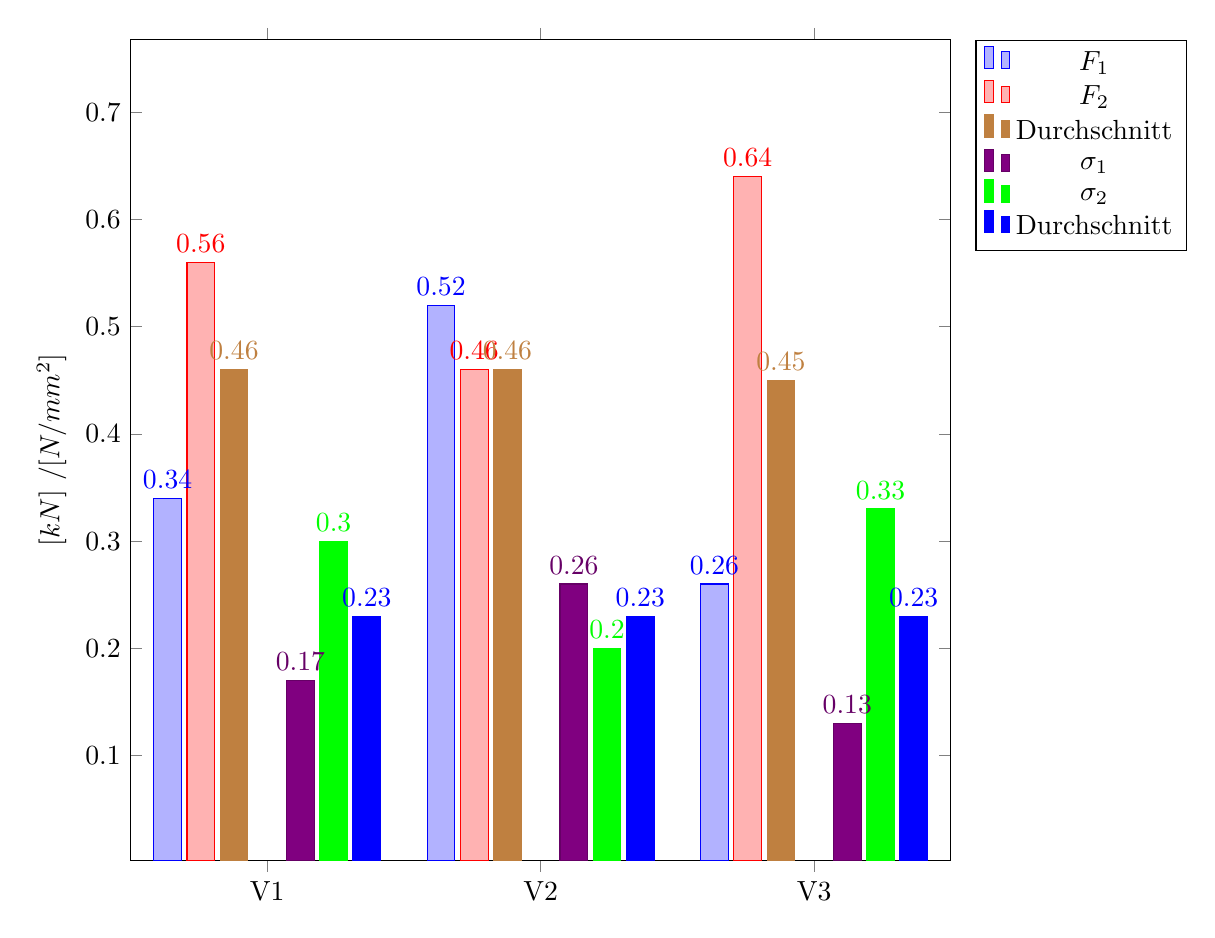
\begin{tikzpicture}
\begin{axis}[legend pos= outer north east,
			height=12cm, width=12cm,
			ylabel= $\lbrack kN\rbrack $ /$\lbrack N/mm^2\rbrack $,
			ybar,
			enlargelimits=0.25,
			symbolic x coords={V1,V2,V3},
			xtick=data,
			nodes near coords
			]
\addplot coordinates {(V1,0.34) (V2,0.52) (V3,0.26)};
\addplot coordinates {(V1,0.56) (V2,0.46) (V3,0.64)};
\addplot [color=brown,fill=brown]coordinates {(V1,0.46) (V2,0.46) (V3,0.45)};
\addplot coordinates {(V1,) (V2,) (V3,)};
\addplot coordinates {(V1,0.17) (V2,0.26) (V3,0.13)};
\addplot[color=green,fill=green]coordinates {(V1,0.30) (V2,0.20) (V3,0.33)};
\addplot[color=blue,fill=blue] coordinates {(V1,0.23) (V2,0.23) (V3,0.23)};
\legend{$F_{1}$,$F_{2}$,Durchschnitt,$ \sigma_{1}$,$ \sigma_{2}$,Durchschnitt}
\end{axis}
\end{tikzpicture}
\caption{Daststellung der Kleberversuchsreihe\,2, Velox: Kraft und Spannung}
\label{BT3}
\end{center}
\end{figure}

\paragraph{Fazit:}

Die Versuchsergebnisse weisen eine starke Streuung auf. Bei Versuch V3 beträgt der Messwert der zweiten Probe mehr als das Doppelte der ersten Messung. Hier ist auch ersichtlich, für die Haftzugversuche mit Velox, dass bei jeder Probe die innere Festigkeit des Velox zu gering war. 
